\section{Experiments}
\label{sec:experiments}

This section describes the experiments carried out to test our implementation of the failure detection algorithm and what we analyse in order to find the best parameters to use with the algorithm.

Apart from some experiments regarding Push and Push-Pull strategy comparison, all the experiments are performed using a $T_{gossip}$ value of $200 \si{ms}$.

In every experiment (except experiments related to catastrophic scenarios) a single node simulates a crash after a certain period of time and the other nodes have to detect it.

All experiments have a duration of 2 minutes and are repeated using the Push and the Push-Pull gossip strategy.

The first experiments have the aim to understand how the failure detector behaves using different values of  $T_{fail}$ and to discover in which conditions the algorithm performs better.
For this experiments, we use 10, 30 and 50 nodes respectively and different strategies to choose the node to which gossip to.
In the following experiments we decide to use only 50 nodes since we notice that the algorithm scales well (the number of involved nodes does not significantly influence the results).

Next, we focus our attention on how the algorithm behaves in catastrophic conditions.
We run the algorithm simulating a catastrophic event: after a certain period of time, \nicefrac{2}{3} of the nodes belonging to the system crash at the same time.
We perform some experiments to observe how the gossip algorithm behaves in these conditions in combination with the multicast backup protocol.
We also use these experiments to empirically find out a proper value for the $T_{miss}$ parameter.

Finally, some experiments are carried out to understand how the use of different $T_{gossip}$ values for different gossip strategies could influence the failure detection algorithm.


\subsection*{Behaviour with respect to $T_{fail}$}

\begin{figure}[t]
	\centering
	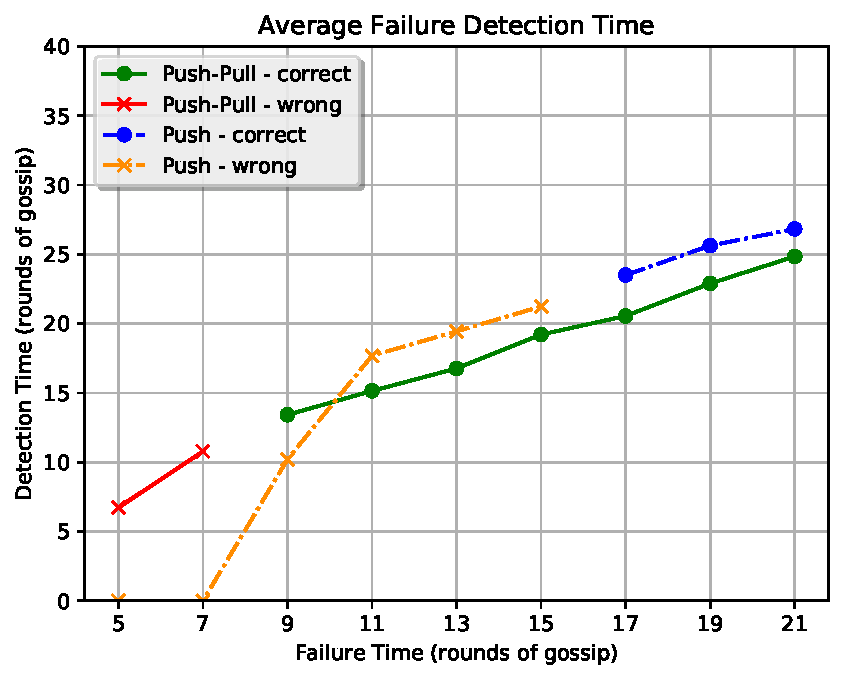
\includegraphics[width=\columnwidth]{figures/n50__average__s0__no_catastrophe__no_multicast}
	\caption{The plot shows the performances of the protocol in case crash of a single out of $50$ nodes. The multicast backup protocol in not enabled. Nodes choose their peers randomly (original strategy) and gossip every $200 \si{ms}$. The Push-Pull variant seems to have better performances for the same values of $T_{fail}$.}
	\label{fig:n50__average__s0__no_catastrophe__no_multicast}
\end{figure}

\cref{fig:n50__average__s0__no_catastrophe__no_multicast} shows correctness and average detection time with varying $T_{fail}$, expressed in terms of gossip intervals.
These experiments clearly show that $T_{fail}$ values under a certain threshold are not suitable.
Since the algorithm is highly probabilistic, even high values of $T_{fail}$ may cause a false detection; in practice, this never happens.
The experiments employing the Push-Pull variant start to behave correctly at a $T_{fail}$ that is roughly half of the one required by Push.
Additionally, average detection time is slightly lower.

High detection times are caused by heartbeat updates that are still circulating in the network after the node crashed.
Since the information spreads faster with Push-Pull, the last node is infected earlier and consequently the detection time lowers.
Some experiments with low $T_{fail}$ are shown with average detection time of 0: this means that there is not even a single correct detection.
There is not enough time for the Push version to gossip with the whole network: nodes start to report each other as crashed.
Even though the actually crashed node is reported, this happened before the actual crash time.


\subsection*{Catastrophe}

\begin{figure}[t]
	\centering
	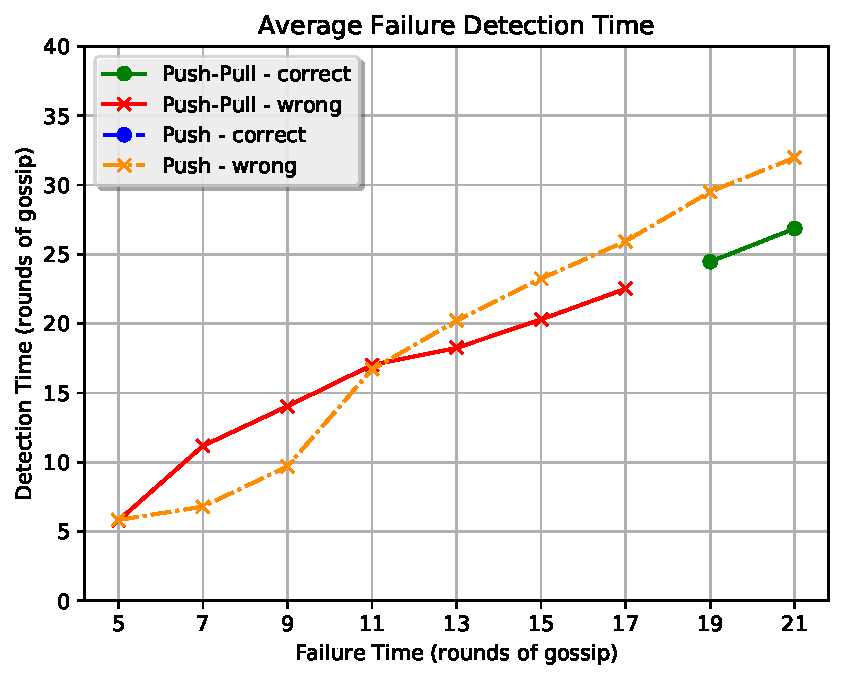
\includegraphics[width=\columnwidth]{figures/n50__average__s0__catastrophe__no_multicast}
	\caption{The plot shows the performances of the protocol in case of the sudden crash of $34$ of $50$ nodes. The multicast backup protocol in not enabled. Nodes choose their peers randomly (original strategy) and gossip every $200 \si{ms}$. The Push variant always fail to correctly report all and only the real crashes. The push-pull variant seems to work with high values of $T_{fail}$.}
	\label{fig:n50__average__s0__catastrophe__no_multicast}
\end{figure}

Some of the experiments are performed to understand how the failure detector behaves when the status of the system suddenly changes.
In particular, we try to understand if the failure detector keeps working correctly (it behaves as a perfect detector) even when \nicefrac{2}{3} of the nodes of the system crash simultaneously. 

As we expected, the failure detector is unable to report crashes correctly with reasonable $T_{fail}$ values.
In catastrophic scenarios, a node has not enough time to update its information about the status of the other nodes before the fixed timeout.
Survived nodes will push their information to crashed nodes wasting the message.
They will not be able to understand who survived the catastrophe before their respective fail timeouts are triggered, reporting also correct nodes as crashed.

\cref{fig:n50__average__s0__catastrophe__no_multicast} shows the Push-Pull strategy with high values of $T_{fail}$ detected crashed nodes without false positives. However, following repetitions of the experiment with the same and higher values of $T_{fail}$ shows that this is not always the case:
in most cases the failure detector does not work correctly despite the high $T_{fail}$.

\begin{figure}[t]
	\centering
	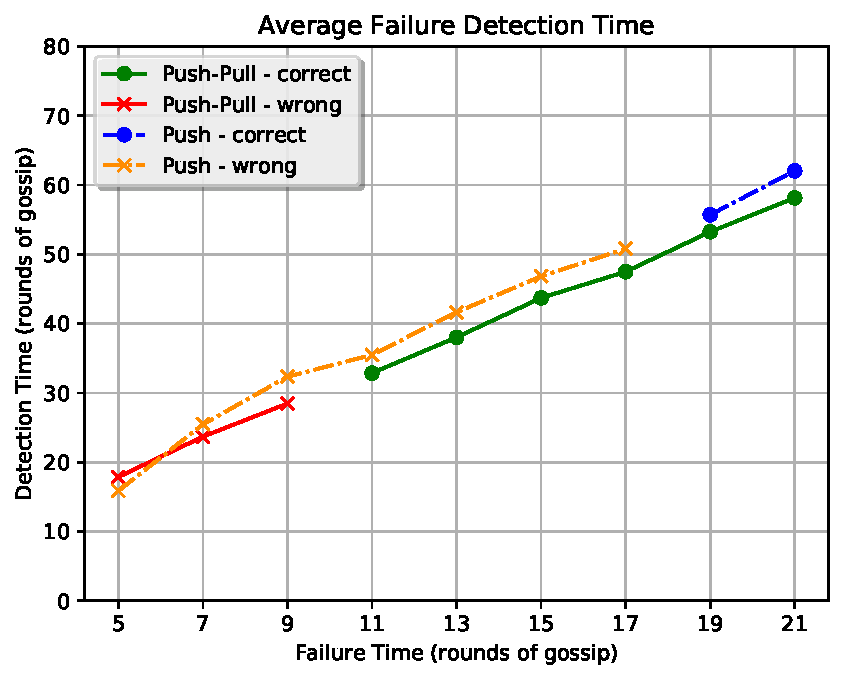
\includegraphics[width=\columnwidth]{figures/n50__average__s0__catastrophe__multicast}
	\caption{The plot shows the performances of the protocol using multicast in case of the sudden crash of $34$ of $50$ nodes. Nodes choose their peers randomly (original strategy) and gossip every $200 \si{ms}$. Thanks to the multicast, also the Push variant starts performing correct detections for high values of $T_{fail}$.}
	\label{fig:n50__average__s0__catastrophe__multicast}
\end{figure}

The strategies to select a node to gossip with described in \cref{sec:variants} are particularly detrimental for the failure detector in this case.
Since the strategies consist in picking the nodes not heard about for a long time with higher probabilities, a node will try to contact exactly the crashed ones. This exacerbates the problem of wasted messages.

To deal with this kind of situation, additional time is granted ($T_{miss}$) so that survived nodes have the chance to find each other.
To ensure that an updated version of heartbeat counters exists, the multicast protocol is used.
The performances are shown in \cref{fig:n50__average__s0__catastrophe__multicast}.
The multicast protocol allows a node to quickly collect information about survived ones after a catastrophe.
This also causes the reset of timers of correct nodes and avoids false positives.

Catastrophe recovery comes with a cost in terms of detection time.
From the comparison of \cref{fig:n50__average__s0__no_catastrophe__no_multicast} and \cref{fig:n50__average__s0__catastrophe__multicast} one notices that the time to detect correctly a fail node approximately doubles for the same $T_{fail}$.
This depends on the fact that the algorithm awaits $T_{miss}$ time after that $T_{fail}$ time is occurred before considering a node as failed. In the experiments proposed in the figures, a $T_{miss}$ equal to $T_{fail}$ has been used.
Due to the slow dissemination caused by the catastrophe, one can expect the average detection time in that case to be even more skewed towards high values.

One can set a $T_{fail}$ value based on the requirements of the system for correctness, balancing detection time and accuracy for specific needs, and the number of crashed nodes the system should tolerate without catastrophe recovery.
$T_{miss}$ is the next parameter to be defined.


\subsection*{Behaviour with respect to $T_{miss}$}

Since after a catastrophe the number of participating nodes decreases,
gossip messages will not take longer than $T_{fail}$ to spread with the same probability as before.
By setting $T_{miss} = T_{fail}$, the information obtained from the multicast protocol should have enough time to travel through all the remaining nodes.
However, we can make the case of the following problematic scenario. One node A is about to report another that is correct, when catastrophe happens. Theoretically, it may take too much time before gossips from the multicast protocol infects A. We argue that a mild catastrophe does not hinder normal functioning enough to result in that scenario, and on the other hand a more severe one would still require less than $T_{miss}$ to spread the information among surviving members.

\begin{figure}[t]
	\centering
	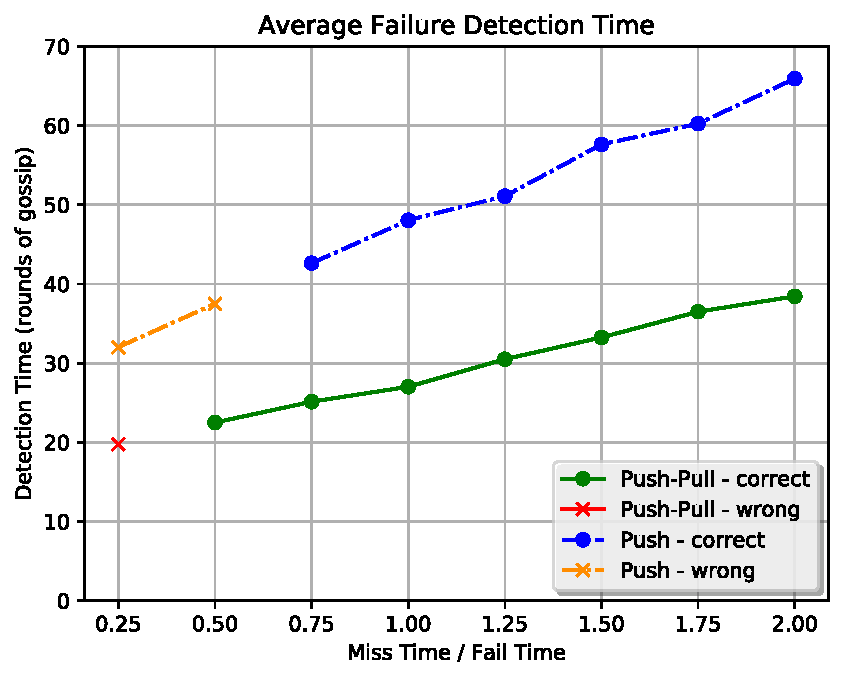
\includegraphics[width=\columnwidth]{figures/n50__miss_times}
	\caption{The plot shows the performances of the protocol using multicast in case of the sudden crash of $34$ of $50$ nodes for different $T_{miss}$. The experiment is performed with a $T_{fail}$ equals to $11$ rounds of gossip for the Push-Pull strategy and $19$ for the Push one. Nodes choose their peers randomly (original strategy) and gossip every $200 \si{ms}$.}
	\label{fig:n50__miss_times}
\end{figure}

Our experiments confirm this hypothesis.
\cref{fig:n50__miss_times} show the behaviour of the protocol in catastrophic conditions for a fixed $T_{fail}$ ($11$ rounds of gossip for the Push-Pull strategy and $19$ for the Push one).
For both strategy, $T_{miss} = T_{fail}$ gives a perfect failure detector.
$T_{miss} = 0.75 \cdot T_{fail}$ seems also to work in both cases, but does not provided a significant boost in the performances.
Since we want the algorithm to be very resilient even in catastrophic situations, we suggest to be slightly more conservative and simply use $T_{miss} = T_{fail}$.
The performances of the protocol can be tuned by changing $T_{fail}$ instead, depending on the real case scenario.


\subsection*{Push vs. Push-Pull}

As described at the beginning of this section, all the experiments are performed using the Push and Push-Pull gossip strategies with a fixed $T_{gossip}$ value of $200 \si{ms}$.
The failure detection algorithm that uses the Push-Pull approach performs always better than the algorithm that use Push.
Such a comparison in not completely fair.

With the Push strategy, each node receives an update on average one time in each round of gossip.
In particular, the expected number of updates can be computed as the probability to be chosen from a node multiplied by the number of nodes in the system.
Since the probability to pick a node has a uniform distribution, the expected number of updated for each node for each round of gossip is exactly one.

In the Push-Pull strategy, a node replies to the sender when it receives an update.
So, a node gets an update in 2 cases: every time it gossips with a not-crashed node and when it is chosen as a peer.
Since we assume independent crashes, we can approximate the probability to gossip with alive node to $1$.
This gives an expected number of updates for each round of gossip equals to roughly $2$.

% When the failure detector algorithm adopts the Push strategy, a node updates another one sending its list of nodes' heartbeats every $T_{gossip}$ (200 \si{ms} in our experiments) and receives information from another node with a probability of 1- Pmistake (?) as described in the paper.

% With the adoption of the Push-Pull strategy, a node that gossips has the opportunity to receive new information also from the node that it contacted (if it is not a crashed one) increasing the probability of the node of obtaining new information in a round of gossip. Therefore, when Push-Pull strategy is used, we can say that almost every $T_{gossip}$ time a node performs a Push and sends its information to other nodes two times: the first time when it contacts a random node with which gossip to and the second time when it replies to an incoming Push-Pull request from another node. 

To evaluate if the Push-Pull strategy really gives an advantage, we perform some experiments halving the $T_{gossip}$ time of the ``Push strategy'' experiments with respect to the $T_{gossip}$ time of the ``Push-Pull strategy'' ones.
We set a $T_{gossip}$ value of $200 \si{ms}$ for the experiments using Push and a $T_{gossip}$ of $400 \si{ms}$ for the experiments using Push-Pull.
The results reveals that the failure detection algorithm adopting the Push-Pull performs still better than the Push one even when its $T_{gossip}$ value is doubled.
A similar experiment with $T_{gossip} = 100 \si{ms}$ for Push and $T_{gossip} = 200 \si{ms}$ for Push-Pull yields the same results.
Comparison experiments have varying $T_{fail}$ (number of rounds corresponding to the same $T_{fail}$ differs between Push and Push-Pull since they have two different $T_{gossip}$). The Push-Pull variant remains correct with $11$ rounds, Push with $23$; Push-Pull obtains slightly lower average detection times as previously observed. Push-Pull can be used with node selection strategies (to obtain updates from quiescent members).

\subsection*{Node selection strategies}

If a node's timeout is approaching, it makes sense to contact it in a Push-Pull fashion to obtain its heartbeat counter. 
It comes out implementing a non-random choice does not allow for significantly lower $T_{fail}$ values. We did not observe improvements in that sense.
If the system can tolerate false positives favouring detection time, strategies seem to help to achieve greater accuracy.
In any case, the benefits of selection strategies were not substantial and not consistent (for consistency, longer experiments are required).
With 50 nodes, strategies did not make any significant impact on the performance.

